% !TeX spellcheck = en_US
%\documentclass[11pt,a4paper]{article}
\documentclass[11pt
  , a4paper
  , article
  , oneside
%  , twoside
%  , draft
]{memoir}

\usepackage{control}
\usepackage[numbers]{natbib}


\begin{document}

\newcommand{\technumber}{
  RAON Control-Document Series\\
  Revision : v1.0,   Release : 2014-12-24 fixed date}
\title{\textbf{Windows OS 상에서 EPICS IOC 구성 방법}}

\author{이상일\thanks{silee7103@ibs.re.kr} \\

  Rare Isotope Science Project\\
  Institute for Basic Science, Daejeon, South Korea
}
\date{\today}

\renewcommand{\maketitlehooka}{\begin{flushright}\textsf{\technumber}\end{flushright}}
%\renewcommand{\maketitlehookb}{\centering\textsf{\subtitle}}
%\renewcommand{\maketitlehookc}{C}
%\renewcommand{\maketitlehookd}{D}

\maketitle

\begin{abstract}
RAON accelerator는 대형 실험 장치로 많은 실험 장치들과 부대시설 장치로 구성되어 운영된다. 이러한 많은 실험 장치들을 제어하기 위한 제어 시스템들은 넓은 범위로 분산되어 구성되어 있으며 이러한 분산 환경에서의 많은 제어시스템들을 전체의 하나의 제어시스템으로 운영하기 위하여 RAON control system은 EPICS software framework을 사용한다. 본 문서는 EPICS가 플랫폼에 독립적으로 운영될 수 있는 환경으로 Windows 운영체제 상에서 구성 방법을 기술한다. 
\end{abstract}

RAON accelerator에서 각 로컬 제어 시스템과 EPICS framework간의 integration을 위하여 가장 핵심이 되는 부분은 EPICS IOC 개발이다. 그만큼 EPICS의 여러 모듈 중에서 IOC는 그 핵심 모듈이라고 할 수 있다. IOC 모듈 구성은 제어시스템의 목적에 따라 개발되며, 여러형태의 하드웨어상에서 운영되어진다. 하드웨어는 개발업체의 특성에 따라 여러 형태의 운영체제 상에서 동작한다. 따라서 해당 제어시스템에 대한 EPICS integration은 하드웨어가 지원하는 운영체제의 software driver의 존재여부가 매우 중요하며 이에 대한 표준화가 필요하다. 이러한 표준화에도 불구하고 제어특성상에서 범용적으로 사용되고 있는 Windows OS상에서만 동작하는 하드웨어가 존재할 수 있다. RAON 가속기 제어시스템에서 사용하고 있는 표준화된 OS는 데비안 리눅스를 사용하며, 하드웨어 특성에 따라 필수 불가결한 경우 Windows OS를 사용 할 수 있는 경우에 EPICS integration을 위하여 Windows OS 상에서 EPICS를 구성하는 방법에 대하여 자세히 언급한다.

\clearpage


\chapter{구성 Software Components}

EPICS는 open source이며, 이런 목적에 따라 Windows OS에 구성을 위하여 open source의 개발 환경을 구성한다.
개발환경에 필요한 software components는 아래와 같다.

\begin{itemize}
	\item Compilers : Microsoft Visual Studio/C++ Express or MinGW (gcc compiler)
	Download URL: C++ Express(Microsoft Homepage), MinGW(http://sourceforge.net/projects/mingw-w64/files/mingw-w64-install.exe)
	\item Build tools : Perl (Strawberry Perl or ActiveState Perl),	Gnu Make
	Download URL: GnuWin:http://sourceforge.net/projects/getgnuwin32/files/GetGnuWin32-0.6.3.exe, 
	Strawberry perl: http://strawberryperl.com/
	\item ConsoleZ : https://github.com/cbucher/console/wiki/Downloads
	\item EPICS Base : base-3.14.12.4(http://www.aps.anl.gov/epics/base/R3-14/12.php)
\end{itemize}

\chapter{Software 설치}
상위 항목에 열거된 software components 항목을 차례로 설치한다. 단, Install 프로그램으로 설치되지 않는 프로그램의 경우는 해당 프로그램의 실행 경로를
Path 환경 변수에 아래와 같이 추가한다.

\begin{figure}[h!]
	\centering
	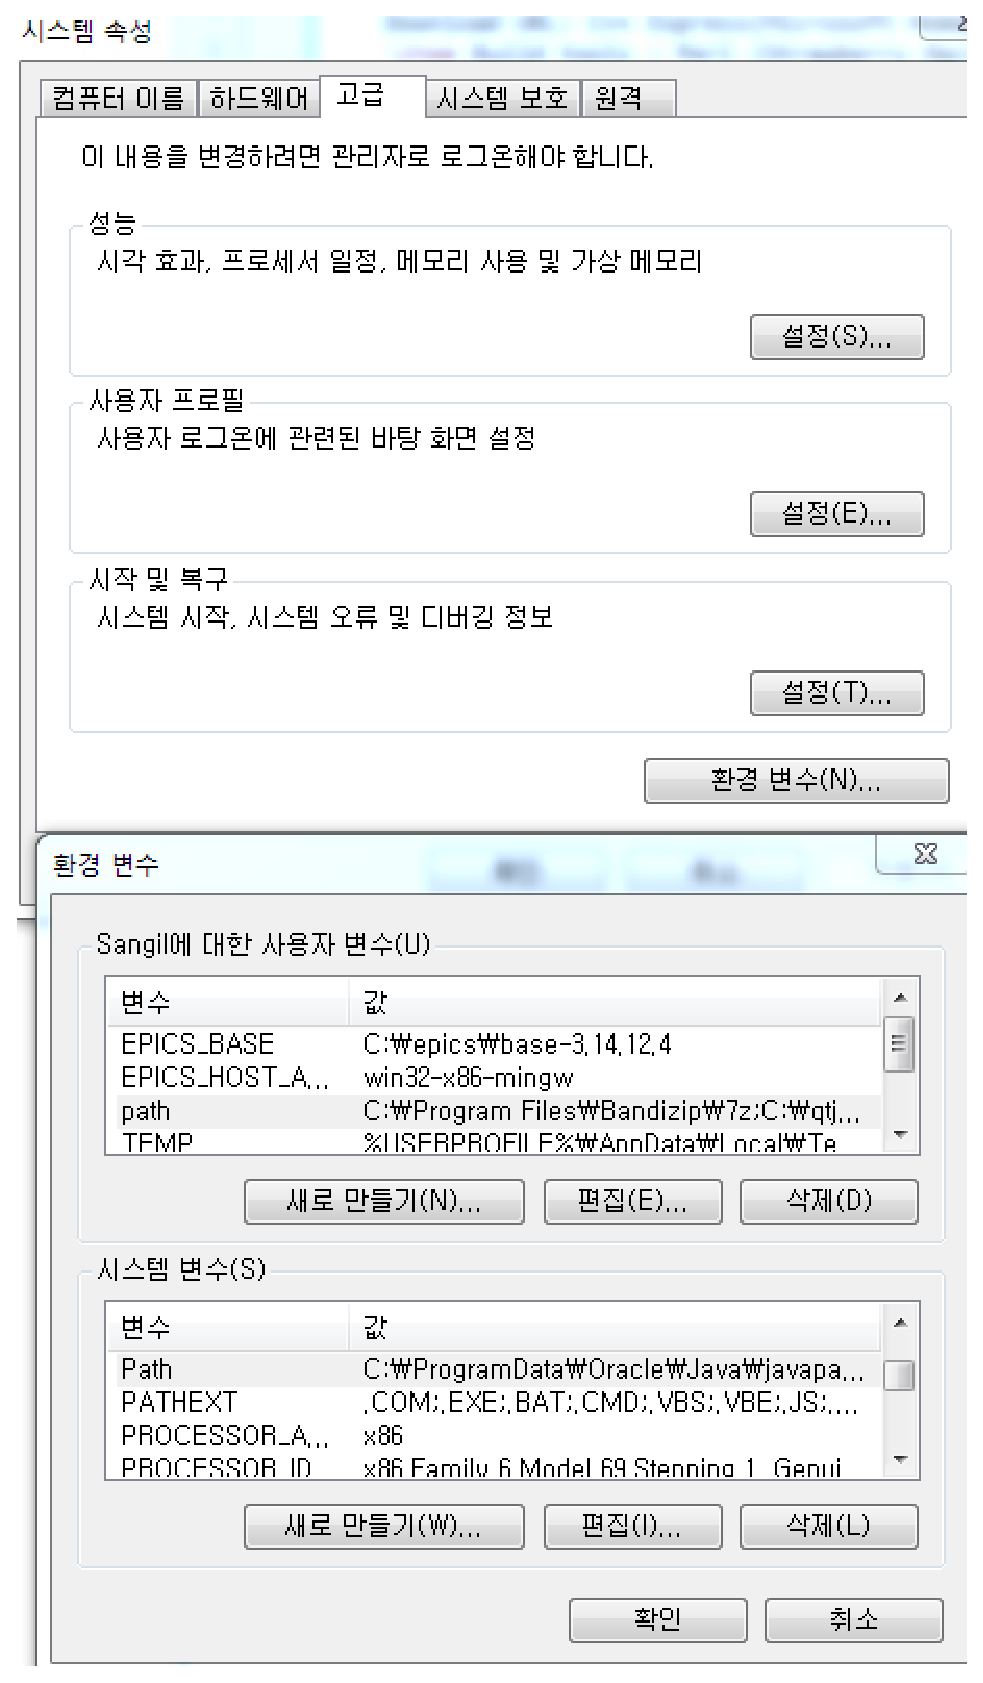
\includegraphics[width=0.55\textwidth, height=0.6 \textwidth ]{./images/env_path.eps}
	\caption{환경변수}
	\label{fig:env_path} 
\end{figure}

상위 항목 중 GnuWin 설치시 생성되는 "libintl3.dll", "libiconv2.dll" 등의 파일은 dll path 설정 또는 "Windows\//System32" 폴더에 복사한다.

그림 \ref{fig:env_path}와 같이 EPICS base 설치를 위한 환경변수 생성은 아래와 같이 한다.
\begin{lstlisting}[style=termstyle]
EPICS_BASE=c:\epics\base-3.14.12.4\
EPICS_HOST_ARCH=win32-x86-mingw
\end{lstlisting}

\chapter{EPICS base build on Windows OS}
EPICS base 설치 경로는 "c:/epics/base-3.14.12.4/" 경로에 설치하며, "configure/os/CONFIG\_SITE" 파일을 아래와 같이 수정한다.

\begin{lstlisting}[style=termstyle]

#  If only a subset of the host architectures perform
#  the build for the CROSS_COMPILER_TARGET_ARCHS
#  uncomment the following line and specify them.
#
CROSS_COMPILER_HOST_ARCHS=win32-x86-mingw 
\end{lstlisting}

EPICS base가 설치된 경로에서 "make", "make install"를 수행하여 아래와 같이 이상없음을 확인한다. 

\begin{lstlisting}[style=termstyle]
C:\epics\base-3.14.12.4>make
make -C ./configure install
make: Entering directory `C:/epics/base-3.14.12.4/configure'
make -C O.win32-x86-mingw -f ../Makefile TOP=../.. T_A=win32-x86-mingw install
make: Entering directory `C:/epics/base-3.14.12.4/configure/O.win32-x86-mingw'
make[2]: Leaving directory `C:/epics/base-3.14.12.4/configure/O.win32-x86-mingw'
make[1]: Leaving directory `C:/epics/base-3.14.12.4/configure'
make -C ./src install
make[1]: Entering directory `C:/epics/base-3.14.12.4/src'
make -C ./tools install
make[2]: Entering directory `C:/epics/base-3.14.12.4/src/tools'
make -C O.win32-x86-mingw -f ../Makefile TOP=../../.. T_A=win32-x86-mingw install
make[3]: Entering directory `C:/epics/base-3.14.12.4/src/tools/O.win32-x86-mingw'
make[3]: Leaving directory `C:/epics/base-3.14.12.4/src/tools/O.win32-x86-mingw'
make[2]: Leaving directory `C:/epics/base-3.14.12.4/src/tools'
make -C ./makeBaseApp install
make[2]: Entering directory `C:/epics/base-3.14.12.4/src/makeBaseApp'
make -C O.win32-x86-mingw -f ../Makefile TOP=../../.. T_A=win32-x86-mingw install
make[3]: Entering directory `C:/epics/base-3.14.12.4/src/makeBaseApp/O.win32-x86-mingw'
make[3]: Leaving directory `C:/epics/base-3.14.12.4/src/makeBaseApp/O.win32-x86-mingw'
make[2]: Leaving directory `C:/epics/base-3.14.12.4/src/makeBaseApp'
make -C ./makeBaseExt install
make[2]: Entering directory `C:/epics/base-3.14.12.4/src/makeBaseExt'
make -C O.win32-x86-mingw -f ../Makefile TOP=../../.. T_A=win32-x86-mingw install
make[3]: Entering directory `C:/epics/base-3.14.12.4/src/makeBaseExt/O.win32-x86-mingw'
make[3]: Leaving directory `C:/epics/base-3.14.12.4/src/makeBaseExt/O.win32-x86-mingw'
make[2]: Leaving directory `C:/epics/base-3.14.12.4/src/makeBaseExt'
make -C ./libCom install
make[2]: Entering directory `C:/epics/base-3.14.12.4/src/libCom'
make -C O.win32-x86-mingw -f ../Makefile TOP=../../.. T_A=win32-x86-mingw install
make[3]: Entering directory `C:/epics/base-3.14.12.4/src/libCom/O.win32-x86-mingw'
make[3]: Leaving directory `C:/epics/base-3.14.12.4/src/libCom/O.win32-x86-mingw'
make[2]: Leaving directory `C:/epics/base-3.14.12.4/src/libCom'
make -C ./toolsComm install
make[2]: Entering directory `C:/epics/base-3.14.12.4/src/toolsComm'
make -C ./antelope install
make[3]: Entering directory `C:/epics/base-3.14.12.4/src/toolsComm/antelope'
make -C O.win32-x86-mingw -f ../Makefile TOP=../../../.. T_A=win32-x86-mingw install
make[4]: Entering directory `C:/epics/base-3.14.12.4/src/toolsComm/antelope/O.win32-x86-mingw'
make[4]: Leaving directory `C:/epics/base-3.14.12.4/src/toolsComm/antelope/O.win32-x86-mingw'
make[3]: Leaving directory `C:/epics/base-3.14.12.4/src/toolsComm/antelope'
make -C ./flex install
make[3]: Entering directory `C:/epics/base-3.14.12.4/src/toolsComm/flex'
make -C O.win32-x86-mingw -f ../Makefile TOP=../../../.. T_A=win32-x86-mingw install
make[4]: Entering directory `C:/epics/base-3.14.12.4/src/toolsComm/flex/O.win32-x86-mingw'
make[4]: Leaving directory `C:/epics/base-3.14.12.4/src/toolsComm/flex/O.win32-x86-mingw'
make[3]: Leaving directory `C:/epics/base-3.14.12.4/src/toolsComm/flex'
make[2]: Leaving directory `C:/epics/base-3.14.12.4/src/toolsComm'
make -C ./ca install
make[2]: Entering directory `C:/epics/base-3.14.12.4/src/ca'
make -C O.win32-x86-mingw -f ../Makefile TOP=../../.. T_A=win32-x86-mingw install
make[3]: Entering directory `C:/epics/base-3.14.12.4/src/ca/O.win32-x86-mingw'
make[3]: Leaving directory `C:/epics/base-3.14.12.4/src/ca/O.win32-x86-mingw'
make[2]: Leaving directory `C:/epics/base-3.14.12.4/src/ca'
make -C ./dbStatic install
make[2]: Entering directory `C:/epics/base-3.14.12.4/src/dbStatic'
make -C O.win32-x86-mingw -f ../Makefile TOP=../../.. T_A=win32-x86-mingw install
make[3]: Entering directory `C:/epics/base-3.14.12.4/src/dbStatic/O.win32-x86-mingw'
make[3]: Leaving directory `C:/epics/base-3.14.12.4/src/dbStatic/O.win32-x86-mingw'
make[2]: Leaving directory `C:/epics/base-3.14.12.4/src/dbStatic'
make -C ./registry install
make[2]: Entering directory `C:/epics/base-3.14.12.4/src/registry'
make -C O.win32-x86-mingw -f ../Makefile TOP=../../.. T_A=win32-x86-mingw install
make[3]: Entering directory `C:/epics/base-3.14.12.4/src/registry/O.win32-x86-mingw'
make[3]: Leaving directory `C:/epics/base-3.14.12.4/src/registry/O.win32-x86-mingw'
make[2]: Leaving directory `C:/epics/base-3.14.12.4/src/registry'
make -C ./bpt install
make[2]: Entering directory `C:/epics/base-3.14.12.4/src/bpt'
make -C O.win32-x86-mingw -f ../Makefile TOP=../../.. T_A=win32-x86-mingw install
make[3]: Entering directory `C:/epics/base-3.14.12.4/src/bpt/O.win32-x86-mingw'
make[3]: Leaving directory `C:/epics/base-3.14.12.4/src/bpt/O.win32-x86-mingw'
make[2]: Leaving directory `C:/epics/base-3.14.12.4/src/bpt'
make -C ./db install
make[2]: Entering directory `C:/epics/base-3.14.12.4/src/db'
make -C O.win32-x86-mingw -f ../Makefile TOP=../../.. T_A=win32-x86-mingw install
make[3]: Entering directory `C:/epics/base-3.14.12.4/src/db/O.win32-x86-mingw'
make[3]: Leaving directory `C:/epics/base-3.14.12.4/src/db/O.win32-x86-mingw'
make[2]: Leaving directory `C:/epics/base-3.14.12.4/src/db'
make -C ./as install
make[2]: Entering directory `C:/epics/base-3.14.12.4/src/as'
make -C O.win32-x86-mingw -f ../Makefile TOP=../../.. T_A=win32-x86-mingw install
make[3]: Entering directory `C:/epics/base-3.14.12.4/src/as/O.win32-x86-mingw'
make[3]: Leaving directory `C:/epics/base-3.14.12.4/src/as/O.win32-x86-mingw'
make[2]: Leaving directory `C:/epics/base-3.14.12.4/src/as'
make -C ./util install
make[2]: Entering directory `C:/epics/base-3.14.12.4/src/util'
make -C O.win32-x86-mingw -f ../Makefile TOP=../../.. T_A=win32-x86-mingw install
make[3]: Entering directory `C:/epics/base-3.14.12.4/src/util/O.win32-x86-mingw'
make[3]: Leaving directory `C:/epics/base-3.14.12.4/src/util/O.win32-x86-mingw'
make[2]: Leaving directory `C:/epics/base-3.14.12.4/src/util'
make -C ./dbtools install
make[2]: Entering directory `C:/epics/base-3.14.12.4/src/dbtools'
make -C O.win32-x86-mingw -f ../Makefile TOP=../../.. T_A=win32-x86-mingw install
make[3]: Entering directory `C:/epics/base-3.14.12.4/src/dbtools/O.win32-x86-mingw'
make[3]: Leaving directory `C:/epics/base-3.14.12.4/src/dbtools/O.win32-x86-mingw'
make[2]: Leaving directory `C:/epics/base-3.14.12.4/src/dbtools'
make -C ./catools install
make[2]: Entering directory `C:/epics/base-3.14.12.4/src/catools'
make -C O.win32-x86-mingw -f ../Makefile TOP=../../.. T_A=win32-x86-mingw install
make[3]: Entering directory `C:/epics/base-3.14.12.4/src/catools/O.win32-x86-mingw'
make[3]: Leaving directory `C:/epics/base-3.14.12.4/src/catools/O.win32-x86-mingw'
make[2]: Leaving directory `C:/epics/base-3.14.12.4/src/catools'
make -C ./rsrv install
make[2]: Entering directory `C:/epics/base-3.14.12.4/src/rsrv'
make -C O.win32-x86-mingw -f ../Makefile TOP=../../.. T_A=win32-x86-mingw install
make[3]: Entering directory `C:/epics/base-3.14.12.4/src/rsrv/O.win32-x86-mingw'
make[3]: Leaving directory `C:/epics/base-3.14.12.4/src/rsrv/O.win32-x86-mingw'
make[2]: Leaving directory `C:/epics/base-3.14.12.4/src/rsrv'
make -C ./rec install
make[2]: Entering directory `C:/epics/base-3.14.12.4/src/rec'
make -C O.win32-x86-mingw -f ../Makefile TOP=../../.. T_A=win32-x86-mingw install
make[3]: Entering directory `C:/epics/base-3.14.12.4/src/rec/O.win32-x86-mingw'
make[3]: Leaving directory `C:/epics/base-3.14.12.4/src/rec/O.win32-x86-mingw'
make[2]: Leaving directory `C:/epics/base-3.14.12.4/src/rec'
make -C ./misc install
make[2]: Entering directory `C:/epics/base-3.14.12.4/src/misc'
make -C O.win32-x86-mingw -f ../Makefile TOP=../../.. T_A=win32-x86-mingw install
make[3]: Entering directory `C:/epics/base-3.14.12.4/src/misc/O.win32-x86-mingw'
make[3]: Leaving directory `C:/epics/base-3.14.12.4/src/misc/O.win32-x86-mingw'
make[2]: Leaving directory `C:/epics/base-3.14.12.4/src/misc'
make -C ./dev install
make[2]: Entering directory `C:/epics/base-3.14.12.4/src/dev'
make -C ./softDev install
make[3]: Entering directory `C:/epics/base-3.14.12.4/src/dev/softDev'
make -C O.win32-x86-mingw -f ../Makefile TOP=../../../.. T_A=win32-x86-mingw install
make[4]: Entering directory `C:/epics/base-3.14.12.4/src/dev/softDev/O.win32-x86-mingw'
make[4]: Leaving directory `C:/epics/base-3.14.12.4/src/dev/softDev/O.win32-x86-mingw'
make[3]: Leaving directory `C:/epics/base-3.14.12.4/src/dev/softDev'
make -C ./testDev install
make[3]: Entering directory `C:/epics/base-3.14.12.4/src/dev/testDev'
make -C O.win32-x86-mingw -f ../Makefile TOP=../../../.. T_A=win32-x86-mingw install
make[4]: Entering directory `C:/epics/base-3.14.12.4/src/dev/testDev/O.win32-x86-mingw'
make[4]: Leaving directory `C:/epics/base-3.14.12.4/src/dev/testDev/O.win32-x86-mingw'
make[3]: Leaving directory `C:/epics/base-3.14.12.4/src/dev/testDev'
make[2]: Leaving directory `C:/epics/base-3.14.12.4/src/dev'
make -C ./vxWorks install
make[2]: Entering directory `C:/epics/base-3.14.12.4/src/vxWorks'
make -C O.win32-x86-mingw -f ../Makefile TOP=../../.. T_A=win32-x86-mingw install
make[3]: Entering directory `C:/epics/base-3.14.12.4/src/vxWorks/O.win32-x86-mingw'
make[3]: Leaving directory `C:/epics/base-3.14.12.4/src/vxWorks/O.win32-x86-mingw'
make[2]: Leaving directory `C:/epics/base-3.14.12.4/src/vxWorks'
make -C ./RTEMS install
make[2]: Entering directory `C:/epics/base-3.14.12.4/src/RTEMS'
make -C ./base install
make[3]: Entering directory `C:/epics/base-3.14.12.4/src/RTEMS/base'
make -C O.win32-x86-mingw -f ../Makefile TOP=../../../.. T_A=win32-x86-mingw install
make[4]: Entering directory `C:/epics/base-3.14.12.4/src/RTEMS/base/O.win32-x86-mingw'
make[4]: Leaving directory `C:/epics/base-3.14.12.4/src/RTEMS/base/O.win32-x86-mingw'
make[3]: Leaving directory `C:/epics/base-3.14.12.4/src/RTEMS/base'
make[2]: Leaving directory `C:/epics/base-3.14.12.4/src/RTEMS'
make -C libCom/test install
make[2]: Entering directory `C:/epics/base-3.14.12.4/src/libCom/test'
make -C O.win32-x86-mingw -f ../Makefile TOP=../../../.. T_A=win32-x86-mingw install
make[3]: Entering directory `C:/epics/base-3.14.12.4/src/libCom/test/O.win32-x86-mingw'
make[3]: Leaving directory `C:/epics/base-3.14.12.4/src/libCom/test/O.win32-x86-mingw'
make[2]: Leaving directory `C:/epics/base-3.14.12.4/src/libCom/test'
make -C db/test install
make[2]: Entering directory `C:/epics/base-3.14.12.4/src/db/test'
make -C O.win32-x86-mingw -f ../Makefile TOP=../../../.. T_A=win32-x86-mingw install
make[3]: Entering directory `C:/epics/base-3.14.12.4/src/db/test/O.win32-x86-mingw'
make[3]: Leaving directory `C:/epics/base-3.14.12.4/src/db/test/O.win32-x86-mingw'
make[2]: Leaving directory `C:/epics/base-3.14.12.4/src/db/test'
make -C ./softIoc install
make[2]: Entering directory `C:/epics/base-3.14.12.4/src/softIoc'
make -C O.win32-x86-mingw -f ../Makefile TOP=../../.. T_A=win32-x86-mingw install
make[3]: Entering directory `C:/epics/base-3.14.12.4/src/softIoc/O.win32-x86-mingw'
make[3]: Leaving directory `C:/epics/base-3.14.12.4/src/softIoc/O.win32-x86-mingw'
make[2]: Leaving directory `C:/epics/base-3.14.12.4/src/softIoc'
make -C ./gdd install
make[2]: Entering directory `C:/epics/base-3.14.12.4/src/gdd'
make -C O.win32-x86-mingw -f ../Makefile TOP=../../.. T_A=win32-x86-mingw install
make[3]: Entering directory `C:/epics/base-3.14.12.4/src/gdd/O.win32-x86-mingw'
make[3]: Leaving directory `C:/epics/base-3.14.12.4/src/gdd/O.win32-x86-mingw'
make[2]: Leaving directory `C:/epics/base-3.14.12.4/src/gdd'
make -C ./cas install
make[2]: Entering directory `C:/epics/base-3.14.12.4/src/cas'
make -C ./build install
make[3]: Entering directory `C:/epics/base-3.14.12.4/src/cas/build'
make -C O.win32-x86-mingw -f ../Makefile TOP=../../../.. T_A=win32-x86-mingw install
make[4]: Entering directory `C:/epics/base-3.14.12.4/src/cas/build/O.win32-x86-mingw'
make[4]: Leaving directory `C:/epics/base-3.14.12.4/src/cas/build/O.win32-x86-mingw'
make[3]: Leaving directory `C:/epics/base-3.14.12.4/src/cas/build'
make -C ./example install
make[3]: Entering directory `C:/epics/base-3.14.12.4/src/cas/example'
make -C ./directoryService install
make[4]: Entering directory `C:/epics/base-3.14.12.4/src/cas/example/directoryService'
make -C O.win32-x86-mingw -f ../Makefile TOP=../../../../.. T_A=win32-x86-mingw install
make[5]: Entering directory `C:/epics/base-3.14.12.4/src/cas/example/directoryService/O.win32-x86-mingw'
make[5]: Leaving directory `C:/epics/base-3.14.12.4/src/cas/example/directoryService/O.win32-x86-mingw'
make[4]: Leaving directory `C:/epics/base-3.14.12.4/src/cas/example/directoryService'
make[3]: Leaving directory `C:/epics/base-3.14.12.4/src/cas/example'
make[2]: Leaving directory `C:/epics/base-3.14.12.4/src/cas'
make -C ./excas install
make[2]: Entering directory `C:/epics/base-3.14.12.4/src/excas'
make -C O.win32-x86-mingw -f ../Makefile TOP=../../.. T_A=win32-x86-mingw install
make[3]: Entering directory `C:/epics/base-3.14.12.4/src/excas/O.win32-x86-mingw'
make[3]: Leaving directory `C:/epics/base-3.14.12.4/src/excas/O.win32-x86-mingw'
make[2]: Leaving directory `C:/epics/base-3.14.12.4/src/excas'
make -C ./cap5 install
make[2]: Entering directory `C:/epics/base-3.14.12.4/src/cap5'
make -C O.win32-x86-mingw -f ../Makefile TOP=../../.. T_A=win32-x86-mingw install
make[3]: Entering directory `C:/epics/base-3.14.12.4/src/cap5/O.win32-x86-mingw'
make[3]: Leaving directory `C:/epics/base-3.14.12.4/src/cap5/O.win32-x86-mingw'
make[2]: Leaving directory `C:/epics/base-3.14.12.4/src/cap5'
make[1]: Leaving directory `C:/epics/base-3.14.12.4/src'
\end{lstlisting}

Base설치 가 완료 된 후 아래와 같은 명령을 실행하여 base IOC 생성 perl script가 이상없이 작동되는지 확인한다.

\begin{lstlisting}[style=termstyle]
C:\epics\testIoc>makeBaseApp.pl -l
Valid application types are:
caClient
caServer
example
ioc
support
Valid iocBoot types are:
example
ioc

C:\epics\testIoc>
\end{lstlisting}

\chapter{test IOC 구성 및 시험}
EPICS base가 이상없이 작동이 되는지 확인을 위하여 testIOC라는 softIOC를 생성한 후 구동한다.

\begin{lstlisting}[style=termstyle]
C:\epics\testIoc>makeBaseApp.pl -t example example
C:\epics\testIoc>makeBaseApp.pl -i -t example example
Using target architecture win32-x86-mingw (only one available)
The following applications are available:
example
What application should the IOC(s) boot?
The default uses the IOC's name, even if not listed above.
Application name?

C:\epics\testIoc>make
make -C ./configure install
make[1]: Entering directory `C:/epics/testIoc/configure'
perl C:/epics/base-3.14.12.4/bin/win32-x86-mingw/makeMakefile.pl O.win32-x86-mingw ../..
perl -MExtUtils::Command -e mkpath O.Common
make -C O.win32-x86-mingw -f ../Makefile TOP=../.. T_A=win32-x86-mingw install
make[2]: Entering directory `C:/epics/testIoc/configure/O.win32-x86-mingw'
perl C:/epics/base-3.14.12.4/bin/win32-x86-mingw/convertRelease.pl checkRelease
make[2]: Leaving directory `C:/epics/testIoc/configure/O.win32-x86-mingw'
make[1]: Leaving directory `C:/epics/testIoc/configure'
make -C ./exampleApp install
make[1]: Entering directory `C:/epics/testIoc/exampleApp'
make -C ./src install
make[2]: Entering directory `C:/epics/testIoc/exampleApp/src'
perl C:/epics/base-3.14.12.4/bin/win32-x86-mingw/makeMakefile.pl O.win32-x86-mingw ../../..
perl -MExtUtils::Command -e mkpath O.Common
make -C O.win32-x86-mingw -f ../Makefile TOP=../../.. T_A=win32-x86-mingw install
make[3]: Entering directory `C:/epics/testIoc/exampleApp/src/O.win32-x86-mingw'
perl C:/epics/base-3.14.12.4/bin/win32-x86-mingw/makeIncludeDbd.pl base.dbd xxxSupport.dbd dbSubExample.dbd exampleHello.dbd initTrace.dbd exampleIncl
ude.dbd
echo "../O.Common/exampleInclude.dbd : ../Makefile" >> example.dbd.d
"Expanding dbd"
"Installing dbd file ../../../dbd/xxxSupport.dbd"
mkdir ../../../dbd
"Installing created dbd file ../../../dbd/example.dbd"
"Installing dbd file ../../../dbd/xxxRecord.dbd"
echo "../O.Common/xxxRecord.h : ../Makefile" >> xxxRecord.h.d
C:/epics/base-3.14.12.4/bin/win32-x86-mingw/dbToRecordtypeH.exe  -I. -I.. -I../O.Common -I../../../dbd -IC:/epics/base-3.14.12.4/dbd ../xxxRecord.dbd
xxxRecord.h
"Installing generated generic include file ../../../include/xxxRecord.h"
mkdir ../../../include
""
gcc -c             -D_MINGW     -O3   -Wall      -m32    -D_DLL   -MMD -I. -I../O.Common -I. -I.. -I../../../include/os/WIN32 -I../../../include -IC:/
epics/base-3.14.12.4/include/os/WIN32 -IC:/epics/base-3.14.12.4/include       ../xxxRecord.c
""
gcc -c             -D_MINGW     -O3   -Wall      -m32    -D_DLL   -MMD -I. -I../O.Common -I. -I.. -I../../../include/os/WIN32 -I../../../include -IC:/
epics/base-3.14.12.4/include/os/WIN32 -IC:/epics/base-3.14.12.4/include       ../devXxxSoft.c
""
gcc -c             -D_MINGW     -O3   -Wall      -m32    -D_DLL   -MMD -I. -I../O.Common -I. -I.. -I../../../include/os/WIN32 -I../../../include -IC:/
epics/base-3.14.12.4/include/os/WIN32 -IC:/epics/base-3.14.12.4/include       ../dbSubExample.c
""
gcc -c             -D_MINGW     -O3   -Wall      -m32    -D_DLL   -MMD -I. -I../O.Common -I. -I.. -I../../../include/os/WIN32 -I../../../include -IC:/
epics/base-3.14.12.4/include/os/WIN32 -IC:/epics/base-3.14.12.4/include       ../exampleHello.c
""
gcc -c             -D_MINGW     -O3   -Wall      -m32    -D_DLL   -MMD -I. -I../O.Common -I. -I.. -I../../../include/os/WIN32 -I../../../include -IC:/
epics/base-3.14.12.4/include/os/WIN32 -IC:/epics/base-3.14.12.4/include       ../initTrace.c
g++ -o exampleSupport.dll -shared -Wl,--out-implib,exampleSupport.lib -LC:/epics/base-3.14.12.4/lib/win32-x86-mingw       -m32               xxxRecord
.o devXxxSoft.o dbSubExample.o exampleHello.o initTrace.o    -lrecIoc -lsoftDevIoc -lmiscIoc -lrsrvIoc -ldbtoolsIoc -lasIoc -ldbIoc -lregistryIoc -ldb
StaticIoc -lca -lCom      -lws2_32
"Installing shared library ../../../bin/win32-x86-mingw/exampleSupport.dll"
mkdir ../../../bin
mkdir ../../../bin/win32-x86-mingw
"Installing library ../../../lib/win32-x86-mingw/exampleSupport.lib"
mkdir ../../../lib
mkdir ../../../lib/win32-x86-mingw
perl C:/epics/base-3.14.12.4/bin/win32-x86-mingw/registerRecordDeviceDriver.pl ../O.Common/example.dbd example_registerRecordDeviceDriver C:/epics/tes
tIoc > example.tmp
perl -MExtUtils::Command -e mv example.tmp example_registerRecordDeviceDriver.cpp
""
g++ -c             -D_MINGW     -O3   -Wall      -m32    -D_DLL   -MMD -I. -I../O.Common -I. -I.. -I../../../include/os/WIN32 -I../../../include -IC:/
epics/base-3.14.12.4/include/os/WIN32 -IC:/epics/base-3.14.12.4/include       example_registerRecordDeviceDriver.cpp
""
g++ -c             -D_MINGW     -O3   -Wall      -m32    -D_DLL   -MMD -I. -I../O.Common -I. -I.. -I../../../include/os/WIN32 -I../../../include -IC:/
epics/base-3.14.12.4/include/os/WIN32 -IC:/epics/base-3.14.12.4/include       ../exampleMain.cpp
g++ -o example.exe  -LC:/epics/testIoc/lib/win32-x86-mingw -LC:/epics/base-3.14.12.4/lib/win32-x86-mingw       -m32               example_registerReco
rdDeviceDriver.o exampleMain.o    -lexampleSupport -lrecIoc -lsoftDevIoc -lmiscIoc -lrsrvIoc -ldbtoolsIoc -lasIoc -ldbIoc -lregistryIoc -ldbStaticIoc
-lca -lCom
"Installing created file ../../../bin/win32-x86-mingw/example.exe"
make[3]: Leaving directory `C:/epics/testIoc/exampleApp/src/O.win32-x86-mingw'
make[2]: Leaving directory `C:/epics/testIoc/exampleApp/src'
make -C ./Db install
make[2]: Entering directory `C:/epics/testIoc/exampleApp/Db'
perl C:/epics/base-3.14.12.4/bin/win32-x86-mingw/makeMakefile.pl O.win32-x86-mingw ../../..
perl -MExtUtils::Command -e mkpath O.Common
make -C O.win32-x86-mingw -f ../Makefile TOP=../../.. T_A=win32-x86-mingw install
make[3]: Entering directory `C:/epics/testIoc/exampleApp/Db/O.win32-x86-mingw'
"Installing db file ../../../db/dbExample1.db"
mkdir ../../../db
"Installing db file ../../../db/dbExample2.db"
"Installing db file ../../../db/dbSubExample.db"
"Installing db file ../../../db/user.substitutions"
"Installing db file ../../../db/userHost.substitutions"
make[3]: Leaving directory `C:/epics/testIoc/exampleApp/Db/O.win32-x86-mingw'
make[2]: Leaving directory `C:/epics/testIoc/exampleApp/Db'
make[1]: Leaving directory `C:/epics/testIoc/exampleApp'
make -C ./iocBoot install
make[1]: Entering directory `C:/epics/testIoc/iocBoot'
make -C ./iocexample install
make[2]: Entering directory `C:/epics/testIoc/iocBoot/iocexample'
perl C:/epics/base-3.14.12.4/bin/win32-x86-mingw/convertRelease.pl -a win32-x86-mingw -t C:/epics/testIoc envPaths
perl C:/epics/base-3.14.12.4/bin/win32-x86-mingw/convertRelease.pl -a win32-x86-mingw -t C:/epics/testIoc dllPath.bat
make[2]: Leaving directory `C:/epics/testIoc/iocBoot/iocexample'
make[1]: Leaving directory `C:/epics/testIoc/iocBoot'

\end{lstlisting}


\section{testIOC 구동}
testIOC가 이상없이 컴파일 됨을 확인한 후 아래와 같이 구동됨을 최종 확인한다.

\begin{lstlisting}[style=termstyle]
C:\epics\testIoc\iocBoot\iocexample>..\..\bin\win32-x86-mingw\example.exe st.cmd
#!../../bin/win32-x86-mingw/example
## You may have to change example to something else
## everywhere it appears in this file
< envPaths
epicsEnvSet("ARCH","win32-x86-mingw")
epicsEnvSet("IOC","iocexample")
epicsEnvSet("TOP","C:/epics/testIoc")
epicsEnvSet("EPICS_BASE","C:/epics/base-3.14.12.4")
cd C:/epics/testIoc
## Register all support components
dbLoadDatabase "dbd/example.dbd"
example_registerRecordDeviceDriver pdbbase
## Load record instances
dbLoadTemplate "db/userHost.substitutions"
dbLoadRecords "db/dbSubExample.db", "user=SangilHost"
## Set this to see messages from mySub
#var mySubDebug 1
## Run this to trace the stages of iocInit
#traceIocInit
cd C:/epics/testIoc/iocBoot/iocexample
iocInit
Starting iocInit
############################################################################
## EPICS R3.14.12.4 $Date: Mon 2013-12-16 15:51:45 -0600$
## EPICS Base built Feb 10 2015
############################################################################
iocRun: All initialization complete
## Start any sequence programs
#seq sncExample, "user=SangilHost"
epics> dbl
SangilHost:ai1
SangilHost:ai2
SangilHost:ai3
SangilHost:aiExample
SangilHost:aiExample1
SangilHost:aiExample2
SangilHost:aiExample3
SangilHost:aSubExample
SangilHost:calc1
SangilHost:calc2
SangilHost:calc3
SangilHost:calcExample
SangilHost:calcExample1
SangilHost:calcExample2
SangilHost:calcExample3
SangilHost:compressExample
SangilHost:subExample
SangilHost:xxxExample
epics>
\end{lstlisting}

\begin{lstlisting}[style=termstyle]
--Windows OS-- 
C:\>camonitor SangilHost:ai1
SangilHost:ai1                 2015-02-11 13:13:15.511420 0 LOLO MAJOR
SangilHost:ai1                 2015-02-11 13:13:16.512889 1 LOLO MAJOR
SangilHost:ai1                 2015-02-11 13:13:17.510317 2 LOLO MAJOR
SangilHost:ai1                 2015-02-11 13:13:18.523406 3 LOW MINOR
SangilHost:ai1                 2015-02-11 13:13:19.521472 4 LOW MINOR
SangilHost:ai1                 2015-02-11 13:13:20.520856 5
SangilHost:ai1                 2015-02-11 13:13:21.519887 6 HIGH MINOR
SangilHost:ai1                 2015-02-11 13:13:22.519063 7 HIGH MINOR
SangilHost:ai1                 2015-02-11 13:13:23.518236 8 HIHI MAJOR
SangilHost:ai1                 2015-02-11 13:13:24.516808 9 HIHI MAJOR
SangilHost:ai1                 2015-02-11 13:13:25.514250 0 LOLO MAJOR
SangilHost:ai1                 2015-02-11 13:13:26.511705 1 LOLO MAJOR
SangilHost:ai1                 2015-02-11 13:13:27.524754 2 LOLO MAJOR
SangilHost:ai1                 2015-02-11 13:13:28.522223 3 LOW MINOR
SangilHost:ai1                 2015-02-11 13:13:29.520388 4 LOW MINOR
SangilHost:ai1                 2015-02-11 13:13:30.519779 5
SangilHost:ai1                 2015-02-11 13:13:31.519216 6 HIGH MINOR
SangilHost:ai1                 2015-02-11 13:13:32.518583 7 HIGH MINOR
SangilHost:ai1                 2015-02-11 13:13:33.517985 8 HIHI MAJOR
SangilHost:ai1                 2015-02-11 13:13:34.516727 9 HIHI MAJOR
SangilHost:ai1                 2015-02-11 13:13:35.514134 0 LOLO MAJOR
SangilHost:ai1                 2015-02-11 13:13:36.511497 1 LOLO MAJOR
SangilHost:ai1                 2015-02-11 13:13:37.524681 2 LOLO MAJOR
SangilHost:ai1                 2015-02-11 13:13:38.522108 3 LOW MINOR
SangilHost:ai1                 2015-02-11 13:13:39.520260 4 LOW MINOR
SangilHost:ai1                 2015-02-11 13:13:40.521656 5
SangilHost:ai1                 2015-02-11 13:13:41.521142 6 HIGH MINOR
SangilHost:ai1                 2015-02-11 13:13:42.522482 7 HIGH MINOR
SangilHost:ai1                 2015-02-11 13:13:43.521863 8 HIHI MAJOR
SangilHost:ai1                 2015-02-11 13:13:44.520603 9 HIHI MAJOR
SangilHost:ai1                 2015-02-11 13:13:45.518042 0 LOLO MAJOR
SangilHost:ai1                 2015-02-11 13:13:46.515493 1 LOLO MAJOR

--Linux OS--
silee@silee:~$ camonitor SangilHost:ai1
SangilHost:ai1                 2015-02-11 13:17:27.520964 2 LOLO MAJOR
SangilHost:ai1                 2015-02-11 13:17:28.518350 3 LOW MINOR
SangilHost:ai1                 2015-02-11 13:17:29.516448 4 LOW MINOR
SangilHost:ai1                 2015-02-11 13:17:30.515778 5  
SangilHost:ai1                 2015-02-11 13:17:31.515052 6 HIGH MINOR
SangilHost:ai1                 2015-02-11 13:17:32.514374 7 HIGH MINOR
SangilHost:ai1                 2015-02-11 13:17:33.513714 8 HIHI MAJOR
SangilHost:ai1                 2015-02-11 13:17:34.512503 9 HIHI MAJOR
SangilHost:ai1                 2015-02-11 13:17:35.509871 0 LOLO MAJOR
SangilHost:ai1                 2015-02-11 13:17:36.522923 1 LOLO MAJOR
SangilHost:ai1                 2015-02-11 13:17:37.524406 2 LOLO MAJOR
SangilHost:ai1                 2015-02-11 13:17:38.521746 3 LOW MINOR
SangilHost:ai1                 2015-02-11 13:17:39.524970 4 LOW MINOR
SangilHost:ai1                 2015-02-11 13:17:40.524350 5  
SangilHost:ai1                 2015-02-11 13:17:41.523791 6 HIGH MINOR
SangilHost:ai1                 2015-02-11 13:17:42.523276 7 HIGH MINOR
SangilHost:ai1                 2015-02-11 13:17:43.522579 8 HIHI MAJOR
SangilHost:ai1                 2015-02-11 13:17:44.523312 9 HIHI MAJOR
SangilHost:ai1                 2015-02-11 13:17:45.520824 0 LOLO MAJOR
\end{lstlisting}
\clearpage
\bibliographystyle{unsrtnat}
\bibliography{./refs}

\end{document}

